\textbf{Overall narrative should be:}

Dark matter is one of the clearest indications of physics beyond the Standard Model.

The absence of a confirmed WIMP signal motivates complementary searches in lower-mass regions.

LDMX targets light dark matter using a missing-momentum fixed-target strategy.

This requires identifying rare signal-like events in a detector environment where pile-up and backgrounds complicate reconstruction.

Modern ML in HEP is increasingly used for exactly this type of high-dimensional reconstruction and triggering problem.

This thesis explores such an ML-based reconstruction strategy for LDMX.


\subsection{Dark Matter Particle Physics}
\label{sec:dm_particle_physics}


Dark matter is an invisible and hypothetical form of matter that does not interact with electromagnetic radiation. Dark matter is motivated by astronomical studies and these imply that dark matter has a gravitational interaction with normal matter, i.e the matter that is included in the \gls{sm} of particle physics. Yet there are no experiments on Earth that have been able to detect dark matter, prove the creation of dark matter, or prove a theory that explains dark matter at the subatomic level. In cosmology dark matter is a widely accepted explanation for observed gravitational effects of celestial bodies that cannot solely be explained by general relativity and normal matter. The bridge of dark matter in cosmology to particle physics has not been trivial. By modern standards, however, this pressing discrepancy between dark matter's clear presence in cosmology and dark matter's absence in particle physics is perhaps the largest reason for why it is considered one of the largest unsolved problems in modern physics. \cite{bertone2016-history-dark-matter} \cite{cirelli2026-darkmatter} 

This subsection will give the reader a brief historical context to dark matter and its introduction in particle physics, an introduction to the thermal freeze out framework that gives thermal relic dark matter, and lastly a description of the Dark Bremsstrahlung particle interaction that is the basis for the \gls{ldmx}.

\subsubsection{Brief History of the Dark Matter Problem}
\label{sec:history}

https://www.physicsforums.com/insights/knut-lundmark-prehistory-dark-matter/

Dark matter as a concept encapsulates the idea of matter that exists, but cannot be perceived by ordinary means. In that sense, dark matter as a concept has been around for a long time not only in physics, but also in natural philosophy even preceding the scientific framework. \cite{bertone2016-history-dark-matter}

Galileo Galilei (17th century) looked out in space with his telescope and measured that the movement of Jupiter had irregularities, implying the presence of satellites of unseen mass orbiting it. Galileo deduced that Jupiter likely had 4 moons orbiting it, thus explaining the observed phenomenon, even though they were not directly observable with the naked eye. \cite{bertone2016-history-dark-matter}
%Much of Galileo’s work throughout his life questioned the existing framework of natural philosophy and the geocentric model, where the Earth was in the center of the solar system. His work with the telescope would lay the foundation for the heliocentric model, where the Sun is in the center instead, and in time this would replace the geocentric one. 

As physics progressed, and astronomers got new frameworks and better tools to observe the universe, new questions and problems emerged. By the time of the mid 1850’s Newton’s laws of motion and gravity was a well established framework to determine the gravitational mass of celestial bodies. Within this framework physicists like Le Verrier struggled to explain the orbit of Mercury, which led to a hypothesized planet called "Vulcan" that could solve the problem. Vulcan, which one could perhaps call a "dark planet", was invisible because it did not exist; the solution Le Verrier was looking for was not found until Einstein's theory of general relativity of the 20th century in which the orbit of Mercury around the sun could be predicted without anomalies. \cite{bertone2016-history-dark-matter}

These stories acts for us as early analogies to the concept of dark matter. In the frontiers of science, with the newest technology available, new forms of matter may be revealed that were previously invisible, and the existence new invisible matter be implied as well. There is yet not an etymological reference to the word of "dark matter", but the earliest recorded mentions of the word would emerge at the start of the 20th century. \cite{bertone2016-history-dark-matter}

Henri Poincaré wrote in 1906 about “matiére obscure” (dark matter) when discussing Lord Kelvin’s novel idea of modeling the stars of the Milky Way as a gas of particles. Borrowing ideas from thermodynamics and applying it to astronomy, which would later become a foundational framework in astronomy for dark matter studies, gave a relationship between the size of the system and the velocity dispersion of the stars, in which measurements provided an upper limit to the mass of the Milky Way. The upper limit was distinctly higher than the visible amount of stars, and if one would assume the upper limit of mass to be true, then it would imply dark bodies to explain the discrepancy. Poincaré argued that the upper limit and the implied amount of \textit{dark matter} to exceed the amount of shining matter seemed like an unlikely scenario, a conclusion not unlikely to make considering even shining mass can sometimes be dim and faintly visible. \cite{bertone2016-history-dark-matter}

Fritz Zwicky was a Swiss-American astronomer in the 1930's and was a pioneer in the emerging (though not yet widely accepted) field of dark matter. He was the first one to apply the virial theorem from thermodynamics to determine the mass of a galaxy cluster and when he applied it to the velocity dispersion derived from redshift measurements of the Coma galaxy cluster he found an unusually large estimation of mass, since the velocity dispersion was also unusually large. The observed mass of the cluster predicted an average velocity dispersion of 80 km/s, but the observed average velocity dispersion was 1000 km/s. Upon this discovery, Zwicky famously wrote 

\begin{center}
\textit{"If this would be confirmed, we would get the surprising result that dark matter ('dunkle Materie') is present in much greater amount than luminous matter."}
\end{center}

Still today, about 90\% of the mass of the Coma cluster is estimated to consist of dark matter. The Coma galaxy cluster is one of the first most prominent examples of an astronomical gravitational anomaly that implies the presence of invisible dark matter. As for the universe as a whole, it is estimated that dark matter makes up about 84\% of the total mass of the universe. 

In the scope of the latest decades in physics there has undergone a transition of dark matter mainly referring to unseen matter in the universe in the context of astrophysics to also include dark matter in the context of particle physics. The inclusion of dark matter's relevancy in particle physics has not always been accepted by the scientific community. As Bertando et al. describes it, cosmology was considered merely half a century ago something of a ''fringe-science'', due to a perceived lack of little predictive power or testability. 

Today however, dark matter has been attempted to be explained by finding a dark matter particle that could fit into the framework of the \gls{sm}. This shift of dark matter research stems perhaps mainly from the fact that baryonic dark matter is simply not compatible with observations any longer. Baryonic dark matter is normal matter that are not stars or otherwise luminous. Baryonic dark matter solutions to the dark matter problem akin the ones of Galileo’s days of unseen moons of Jupiter are not possible anymore and and the ''unlikely'' possibility of a dark matter exceeding the amount of shining matter of Poincaré's days have become instead the likely scenarios. The exclusion of baryonic dark matter are based on two main observational truths: 

\begin{itemize}
    \item The amount of baryonic matter in (i.e non-luminous normal matter) needed to make up for the missing mass would cause gravitational lensing in a way that is not observed. 
    \item The cosmic microwave background sets an upper limit on the anmount on the baryonic dark matter in the universe, which is 20\% of total universe mass. 
\end{itemize}

There has has also been other attempts of explanations of the dark matter problems, such as finding a new elegenat model of gravity as with the proposed \gls{mond} (Mordehai Milgrom, 1982) that has been one of the leading candidate solutions that found initial success to explain dark matter phenomenon that does not introduce particle dark matter, but there has also been critical observations difficult to merge with \gls{mond}, thus pointing the way for dark matter candidates in particle physics once again. 

This concludes the historic review for the scope of this paper. The roots of dark matter in modern physics is based in astronomy, and the transition from the cosmological scale in astrophysics to the subatomic scale in particle physics has so far proven to be highly nontrivial.

\subsubsection{Dark Matter Particles}
\label{sec:dm_particles}

Over the last decades the arguments for dark matter particles has become the frontier standard and solutions to the dark matter problem is trying to be found in particle physics. Evidence points to the following key properties must hold true for any dark matter particle candidate:

\begin{enumerate}
    \item \textbf{Mass}
    \begin{itemize}
        \item A dark matter candidate must have mass higher than zero. The mass of dark matter is why it has gravitational influence with other matter, including normal matter included in the \gls{sm}. 
    \end{itemize}
    \item \textbf{Stability}
    \begin{itemize}
        \item There is observational evidence for dark matter in the cosmic microwave background. This implies the existence of dark matter to the early stages of the universe, and thus it must be stable enough to have a long lifetime reaching over the current age of the universe.
    \end{itemize}
    \item \textbf{Almost no interaction with the \gls{sm}}
    \begin{itemize}
        \item The only proven interaction of dark matter with the particles of the \gls{sm} is gravity, which is considered to be the weakest interaction within the \gls{sm}, even so weak it is not even experimentally found or explained by \gls{sm} itself. Dark matter has no interaction with the electromagnetic force, and \textbf{\textit{if}} there are any other interactions with the \gls{sm}, then it must be weaker than the interaction strengths already ruled out by experiments. 
    \end{itemize}
\end{enumerate}

\subsubsection{Thermal Relic Dark Matter}
%by a Thermal Freeze-Out Process}
\label{sec:termal_relic}


Thermal relic dark matter posits that the abundance of dark matter in the universe is a relic from the early stage of the universe. The relic dark matter could be explained by a \textit{thermal freeze-out process} and in the thermal freeze-out hypothesis one assumes that the normal matter of the \gls{sm} is an almost entirely separated sector compared to dark matter sector (in line with \textit{3)} from \ref{sec:dm_particles}) where we do not know its particle content. The key part of this hypothesis is that we assume at least some non-gravitational interaction between two sectors exists. Thus, in this hypothesis there exists a ''bridge'' between the two sectors this enables a \textit{coupling} between them, i.e destruction of normal matter to creation of dark matter and vice versa. These are the necessary conditions for the thermal freeze-out process. 

At the early stages of the universe, space was much smaller, and all energy was confined within it, thus implying a high average amount of available energy. These conditions allowed for the creation of mediator particles that coupled the \gls{sm} and the dark matter sectors and these two must thus have been in \textit{thermal equilibrium}. As the universe expanded and cooled down over time, eventually this bridge between the two sectors would close as mediator particles could not be formed and the thermal equilibrium becomes \textit{frozen out}. If dark matter is stable, then the total mass of dark matter from the early stage should be relatively preserved, and this is the \textit{thermal relic dark matter} we observe in the universe today. \cite{du2022-revisiting-freeze-in-freeze-out} 


Thermal equilibrium corresponds to
\[
    \Gamma_\chi = n_\chi^{\mathrm{eq}}\langle\sigma v\rangle \gg H,
\]
which ensures that $n_\chi \simeq n_\chi^{\mathrm{eq}}$. Freeze-out occurs when
\[
    \Gamma_\chi(T_f) \sim H(T_f),
\]
after which the comoving abundance $Y_\chi = n_\chi/s$ no longer tracks
$Y_\chi^{\mathrm{eq}}$.

The thermal freeze out scenario gives a lower and an upper bound on the mass of dark matter particles to XX-XX, which narrows down the search for dark matter particles substantially, please see the energy range in figure \ref{fig:dm_candidate_range}. Within the energy range of thermal dark matter the search for dark matter particles can be even further narrowed down if we restrict the search to the energy range of \gls{ldm}, and this is the energy range of interaction strength that the \gls{ldmx} has narrowed down its search for dark matter candidates by excluding the possibility of the \gls{wimp}. 

\begin{figure}
    \centering
    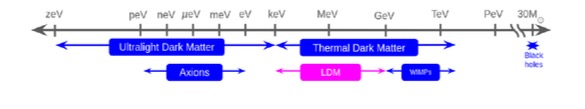
\includegraphics[width=1\linewidth]{config/fig/dm_range.jpeg}
    \caption{Energy ranges of possible DM candidates. Thermal dark matter is in the energy range of XX-XX and the light dark matter energy range is a subset of YY-YY.}
    \label{fig:dm_candidate_range}
\end{figure}




\subsubsection{Dark Bremsstrahlung - A Benchmark Model for LDMX}
\label{sec:dark_brem}

\begin{figure}
    \centering
    
\includegraphics[width=1\linewidth]{dark_brem.jpeg}
    \caption{Enter Caption}
    \label{fig:placeholder}
\end{figure}



\subsection{The Light Dark Matter eXperiment}
\label{sec:ldmx}

\gls{ldmx} is an electron fixed-target experiment in particle physics with the intention to probe for dark matter candidates in the sub-GeV mass range, a sector that is still largely unexplored. 
\gls{ldmx} is designed to search for matter production of the dark bremsstrahlung particle interaction through a
\textit{missing momentum} signature, i.e the experiment will search for a loss of energy that matches an expected dark matter interaction strength for a certain dark matter theoretic model. \gls{ldmx} will operate at the \gls{slac} in San Francisco, California using an 8 GeV electron beam and the design of the experiment is motivated by the performance requirements of a high-rate missing momentum search. The unique angle of \gls{ldmx} for dark matter search is enabling sensitivity to MeV-GeV dark matter interaction strengths, thus expanding dark matter search to new energy regions. \cite{akesson2018-ldmx}

As of the time of writing this report, the international collaboration of design and preparation of the experiment is ongoing and it includes development of different areas of the experiment such as: the detectors and sub-detector electronics but also the implementation of algorithms and other computational methods that determines what measurements that will be stored and that analyzes the data measurements \textit{reconstructing} what physical observables took place in the particle event. This section will cover the different parts of the \gls{ldmx} apparatus and corresponding tools for data storage that are relevant to the scope of this report: the tracker subdetector and the electromagnetic calorimiter subdetector and the trigger. 

\subsubsection{LDMX Search for Dark Matter}

\begin{figure}[H]
    \centering
    
\includegraphics[width=1\linewidth]{exclusion_ldmx.jpeg}
    \caption{\textbf{from Aert} Projected exclusion prospects for the different runs of LDMX. Benchmark thermal
relic targets for DM with different particle properties are shown as black lines, and constraints
from previous experiments are represented by the gray area}
    \label{fig:exclusion_ldmx}
\end{figure}

\subsubsection{Detector Setup}

This subsection should give the reader an overview of the entire LDMX detector where the different subdetectors are clearly laid out. The tracker, 


* Include a figure with schematics of the ldmx detector. 

\begin{figure}[H]
    \centering
    
\includegraphics[width=1\linewidth]{ldmx_schem.jpeg}
    \caption{A schematic layout of the LDMX detector.}
    \label{fig:ldmx_schem}
\end{figure}

* 

\subsubsection{Electromagnetic Calorimiter}

This subsection should cover the ECal subdetector. 

* Include a figure with the ECal cells and the trigger cells of the ECal. 

\subsubsection{Tracker and Trigger Scintillators}

This subsection should cover the tracker subdetector including: trigger scintillators, tracker, recoil tracker. 

* Include a figure with the trigger scintillator schematics. The current one and the newly proposed one as well. 

\subsubsection{Trigger}

Define the trigger and explain + motivate its purpose. 

-> Also introduce the concept of online analysis

\subsubsection{Formalism: electrons and detector response as stochastic variables}
\label{sec:formalism}


Let \(T^{(k)}\) denote the physical trajectory and shower development of electron \(k\). 
The corresponding true energy depositions in the \gls{ecal} are represented by
\[
Z^{(k)} = \{(r^{(k)}_i, E^{(k)}_i)\}_{i=1}^{N_k},
\]
where \(r^{(k)}_i \in \mathbb{R}^3\) is the spatial position of deposition \(i\), 
\(E^{(k)}_i\) is the deposited energy, and \(N_k\) is the number of depositions associated with electron \(k\).

For distinct primary electrons \(k \neq \ell\), the simulated shower developments are treated as independent processes,
\[
T^{(k)} \perp\!\!\!\perp T^{(\ell)}
\]
Consequently, the corresponding true energy deposition patterns are also treated as independent,
\[
Z^{(k)} \perp\!\!\!\perp Z^{(\ell)}
\]

The detector response is represented by a stochastic mapping from true energy depositions to observed or reconstructed detector hits. 
Let
\[
H = \mathcal{R}\!\left(Z^{(1)},\ldots,Z^{(m)}\right)
\]
denote the set of reconstructed \gls{ecal} hits produced after overlay and detector response, where \(\mathcal{R}\) includes effects such as finite detector granularity, energy sharing, thresholds, noise, and reconstruction procedures.

Although the underlying deposition patterns \(Z^{(1)},\ldots,Z^{(m)}\) are treated as independent before overlay, the observed hit collection \(H\) is not naturally decomposed into independent components. After detector response and reconstruction, energy depositions from different electrons may overlap spatially, contribute to the same reconstructed hit, or become difficult to assign uniquely to their originating electron.



\subsubsection{Pile-Up and Physics Reach of LDMX}

Explain what reconstruction is

Explain what pile-up is and \textit{WHY} pile-up is a problem

-> Refer to the concept of online and introduce offline, and what something in between is. 

\subsection{Machine learning for Reconstruction in HEP}
\label{sec:ml_event_reconstruction_hep}


Short introductory text here stating that ML is a topic of rising interest in HEP and refer to output of ML-related papers in HEP. \cite{iml-wg-hepml-livingreview}'


\textbf{text here}

Machine learning has become a tool of rising interest and importance in \gls{hep}, driven by the growing complexity of detector data, the need for efficient event selection, and the search for rare signatures of physics beyond the \gls{sm}. At the same time, advances in deep-learning methods and accelerator-based computing architectures such as \glspl{gpu} have made increasingly powerful \gls{ml} and non-\gls{ml} approaches practical for scientific workflows \cite{sur2026-heterogeneous-computing}. Machine learning and deep-learning methods are not new in \gls{hep}, but the recent rapid growth of machine-learning applications in particle physics is 
\begin{wrapfigure}{r}{0.50\textwidth}
    \centering
    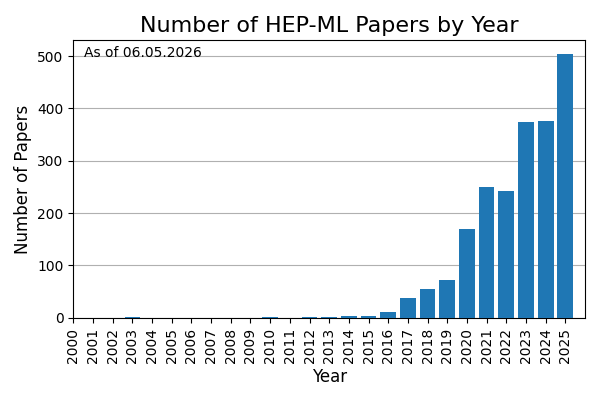
\includegraphics[width=0.48\textwidth]{config/fig/per_year.png}
    \caption{\textbf{Increase the size of labels here} Number of machine-learning-related publications on arXiv in the HEP category per year, based on the Living Review of Machine Learning for Particle Physics \cite{iml-wg-hepml-livingreview}.}
    \label{fig:ml-publications-per-year}
\end{wrapfigure}
reflected both in dedicated reviews and in the continuously updated Living Review of Machine Learning for Particle Physics  \cite{karagiorgi2021-mlnewphysics,feickert2021-livingreview,iml-wg-hepml-livingreview}, please see figure \ref{fig:ml-publications-per-year} that shows the trend of machine-learning-related publications within \gls{hep} significantly increasing in the last few years. 


The underlying motivation for \gls{ml} in \gls{hep} is that such tools may increase the \textit{physics reach} of experiments, meaning their ability to probe weaker signals, rarer processes, or more challenging regions of parameter space, either by improving sensitivity enabling new discoveries or by making reconstruction and selection more computationally efficient. Modern \gls{hep} experiments produce high-dimensional and heterogeneous data, where each event may contain a variable number of detector signals distributed across several subdetectors. This makes reconstruction a natural application area for machine learning: the task is to transform low-level or intermediate detector information, such as hits, tracks, and calorimeter clusters, into physically meaningful quantities that can be used for triggering, event selection, and analysis. \textit{Reconstruction} in \gls{hep} refers to reconstructing the physical interpretables from a measured particle event based on the detector outputs. 



A useful way to view reconstruction is as an approximate inverse problem. In simulation, a detector may be regarded as a map from an underlying particle-level event to a set of detector measurements. If the particle-level event, representing the physical ''truth'', is denoted by \(Y\), and the corresponding detector response by \(X\), the simulation can be written schematically as
\begin{equation}
    S(Y) = X ,
\end{equation}
where \(S\) represents the detector response. Reconstruction then attempts to approximate the inverse mapping,
\begin{equation}
    R(X) \approx S^{-1}(X) = Y .
\end{equation}
In practice, this inverse is imperfect and often ambiguous, based on the fact that some information is always lost or only indirectly observed: detector signals have finite resolution and particles may overlap in the detector. These cases does exclude relevance however as it could be useful to study these scenarios as well. Machine-learning-based reconstruction approaches formulate parts of this inverse problem as a learnable mapping from detector-level inputs to physics-level targets, typically using simulated events where target information is available.

The computational setting of \gls{hep} is also important for understanding the interest in machine-learning-based reconstruction. Large-scale \gls{hep} computing has traditionally been dominated by distributed, \gls{cpu}-based workflows. \cite{sur2026-heterogeneous-computing} This is natural because collision or fixed-target events often are, to a good approximation, independent processes, analog to the electron case of \gls{ldmx} $Z^{(k)} \perp\!\!\!\perp Z^{(\ell)}$ where $k \neq l$, following the notation introduced in Section~\ref{sec:formalism}. Simulation, reconstruction, and analysis can therefore often be parallelized over events with relatively little communication between tasks, making \gls{cpu} clusters and grid computing highly effective, somewhat bypassing an immediate need of software engineering concurrency, which explains the longevity and success of this computing paradigm within \gls{hep}.

At the same time, the wider computing landscape has shifted toward heterogeneous architectures, in particular \glspl{gpu} and other accelerator \footnote{Here, ``accelerator'' refers to specialized hardware such as \glspl{gpu} or even \gls{ml} specialized architectures such as the relatively new \gls{tpu} designed by Google that accelerate the speed of computation for applicable processes\cite{needed}}
-based systems. This development is strongly connected to modern machine learning, where many operations reduce to dense linear algebra and can be executed efficiently on massively parallel hardware, including both training and inference tasks of deep learning \gls{ml} models.

This shift creates both a challenge and an opportunity for \gls{hep}. Rule-based reconstruction algorithms have often been designed around detector-specific logic and sequential or iterative procedures. Such algorithms can be highly effective, but they may be difficult to port efficiently to accelerator hardware and may scale poorly with detector occupancy. Machine-learning models, by contrast, often express reconstruction as a fixed sequence of tensor operations, making inference naturally suited to \glspl{gpu} or other accelerator architectures. This is one of the motivations behind machine-learned particle-flow reconstruction. The original \gls{mlpf} study used a graph-neural-network-based architecture for efficient particle-flow reconstruction in high-pile-up conditions \cite{pata2021-mlpf}. A later \gls{cms} implementation demonstrated a transformer-based \gls{mlpf} algorithm integrated into the \gls{cms} reconstruction software and evaluated on both simulation and collision data \cite{pata2026-mlpf}. In the latter study, modern hardware and transformer-based architectures are explicitly part of the motivation for scalable reconstruction in high-dimensional, variable-size event data.

For the purpose of this thesis, the most relevant role of machine learning is therefore not only as a final classifier that separates signal-like and background-like events, but as a possible reconstruction method. Traditional reconstruction algorithms are often built from physics-motivated rules and detector-specific heuristics. Such methods remain essential, but they may become difficult to optimize in environments with high occupancy, irregular detector geometry, or overlapping detector signatures. Machine-learning-based reconstruction instead attempts to learn parts of the reconstruction mapping $R(X) \approx S^{-1}(X) = Y$ directly from simulated or measured data. This is especially relevant under pile-up conditions, where detector hits from several particles or interactions may overlap and where the association between detector activity and the underlying particle origin becomes ambiguous. In this setting, a model that operates directly on hit-level or object-level detector information may provide additional information beyond a purely rule-based reconstruction, for example by assigning hit-level probabilities or by learning correlations that may be difficult to capture manually with code. 

Architectures such as \glspl{gnn} and transformers are particularly well suited to this type of problem because they can operate on variable-size collections of detector objects and learn correlations between them without requiring the data to be arranged on a regular grid. This is important for particle detectors, where the relevant information is often distributed over irregular detector geometries and across multiple subdetectors. By contrast, architectures such as \glspl{cnn} are naturally adapted to regularly spaced image-like data and therefore impose an inductive bias that is not always well matched to detector readout. Graph-based models instead allow calorimeter hits, clusters, tracks, or other detector objects to be represented as nodes, with edges describing geometrical proximity or learned relationships. Transformers provide a related but distinct approach, where correlations between detector elements are learned through attention rather than through an explicitly constructed sparse graph.

In this thesis, the same general motivation is applied to the \gls{ldmx} setting. The aim is not to perform full general-purpose particle-flow reconstruction, as in \gls{cms}, but to build and study a reconstruction platform for identifying electron-induced activity in the electromagnetic calorimeter, especially under pile-up conditions. This is the regime where reconstruction ambiguities are expected to be most important, and where machine-learning methods may offer the largest benefit over rule-based approaches.

This subsection introduces the machine-learning context needed for the reconstruction study in this thesis. First, the existing rule-based reconstruction chain in \gls{ldmx} is reviewed, with emphasis on clustering, particle-flow-inspired reconstruction, and the distinction between online and offline reconstruction. The existing machine-learning-based veto strategy in \gls{ldmx} is then briefly discussed, since it represents an already planned use of machine learning in the experiment. The subsection then turns to machine-learning-based reconstruction in \gls{cms}, in particular the development of \gls{mlpf}, which provides a useful point of comparison for the approach studied here. Finally, the basic ideas behind \glspl{gnn} and transformers are introduced and compared. These architectures form the methodological basis for representing calorimeter hits and other detector objects as sets or graphs, allowing event reconstruction to be formulated as a learnable mapping from detector-level inputs to physics-level targets.


\subsubsection{Rule-Based Reconstruction in LDMX}

Introduce clustering and reconstruction pipelines. Describe existing LDMX reconstruction approaches (CLUE, PF).

Discuss online vs offline reconstruction context in order to give the reader an idea of online/offline and where this reconstruction method aims to relate.

\subsubsection{ML-based Veto in LDMX}

Briefly explain and overview the particle-net implementation that is in place for LDMX. 

%\subsubsection{CLUE}

%\subsubsection{ParticleFlow}

\subsubsection{ML-based Reconstruction in CMS}

Cover MLPF and ParticleNet here. 

*Figure flowchart of where the different alternatives of reconstruction (Rule based CLUE, PF and ML) fit in the reconstruction pipeline of LDMX*


Beyond physics performance, the \gls{mlpf} studies are relevant because they connect reconstruction algorithms to modern heterogeneous computing. The original graph-based \gls{mlpf} work emphasized scalable graph construction and accelerator-friendly inference \cite{pata2021-mlpf}, while the later \gls{cms} implementation demonstrated that a transformer-based reconstruction model can be integrated into the \gls{cms} software framework and evaluated on \gls{gpu} hardware \cite{pata2026-mlpf}. This makes \gls{mlpf} an example not only of machine-learning-based reconstruction, but also of how reconstruction algorithms may adapt to the changing computational architecture of \gls{hep}.

\subsubsection{The Graph Neural Network}

Explain the prospect of GNN and discuss advantages compared to CNNs/RNNs for irregular geometries.

Explain why calorimeter data can naturally be represented as graphs. Explain how data from other subdetectors can be included in the same graph representation and refer to MLPF by CMS.

Introduce graph representations and message passing.

Explain Graph Convolution

Explain GraphNetConvolution paper \cite{qasim2019-gravnet}

Discuss hit-level vs cluster-level inputs.

Explain graph construction: edge definitions, distance metrics, kNN or radius graphs or perhaps fully connected.

*Figure illustrating input possibilities could be nice here*

\subsubsection{The Transformer}

First give the necessary background to the transformer and the basics of it and how it is structured. 

Very briefly mention the transformer's extreme rise in popularity seen with the rise of LLM and the prediction in the direction of compute architectures.


\subsubsection{Transformer and GNN analogy}

The transformer and the gnn architectures are distinct architectures but they also have similarities and one can mold the gnn to essentially become a transformer: there exist an analogy between them and I believe it is revolved around a fully connected graph gnn is essentially a transformer (but without the self attention mechanism?) and vice versa. Explain how a fully connected graph can be compared to a transformer. Explain a transformer and explain the attention mechanism. What is the stepping stone distance going from a GNN to a transformer? Why could that be reasonable? Does it anticipate to introduce new challenges?



*Figure somewhere illustrating the idea of GNN in HEP reconstruction and subdetector data (probably omit if there is a proper one later anyways)*


